\documentclass[a4paper,12pt,french]{report}
\usepackage[utf8]{inputenc}
\usepackage[T1]{fontenc}
\usepackage{textcomp}
\usepackage{babel}
\usepackage{amsmath,amssymb}
\usepackage{minted}
%\usepackage[toc,pagee]{appendix}
\usepackage{graphicx}
\graphicspath{
	{images}
}
\usepackage{caption}
\usepackage[top=2cm,left=2cm,right=2cm,bottom=2cm,headsep=1.5cm]{geometry}
\usepackage[hidelinks]{hyperref}
\usepackage{xcolor}
\usepackage{bbold}
\usepackage{titlesec}
\usepackage{blindtext}
\usepackage{multicol}

\usepackage{fancyhdr} %en-tetes et bas de page
\pagestyle{fancy}
%\fancyhf{} % Efface les en-têtes et pieds de page par défaut

\usepackage[style=numeric,backend=bibtex, sorting=none]{biblatex}
%\addbibresource{TPMN.bib}

\usepackage{csquotes}

%Outils Mathématiques
\addto\captionsfrench{
    \renewcommand*{\chaptername}{Partie}
}
\newcommand{\N}{\mathbb{N}}
\newcommand{\R}{\mathbb{R}}
\renewcommand{\P}{\mathcal{P}}
\newcommand{\lsum}[2]{\sum\limits_{#1}^{#2}}
\newcommand{\x}{\times}
\renewcommand{\phi}{\varphi}
\renewcommand{\epsilon}{\varepsilon}

\newcommand{\norminf}[1]{\left\lVert {#1} \right\rVert _\infty}
\newcommand{\norm}[1]{\left\lvert {#1} \right\rvert}
\newcommand{\norme}[2]{\left\lVert {#1} \right\rVert_{#2}}


\DeclareMathOperator{\e}{\mathrm e}
\newcommand{\abs}[1]{\lvert#1\rvert}

\newtheorem{theorem}{Théorème}
\newtheorem{propo}{Proposition}
\newtheorem{prop}{Propriété}

% \renewcommand{\bf}{\textbf}

% ON MET DES ACCENTS SUR LES MAJUSCULES
% accent aigu : \' (apostrophe)
% accent grave : \` (accent grave en-dessous de £)
% accent circonflexe : \^
% tréma : \"

%PAGE DE GARDE
\author{Rozenn \textsc{Le Bihan}
\\Axel \textsc{Raynond}
\\Rémy \textsc{Labarre}
\\Matys \textsc{Bieche}
\\Alexandre \textsc{Amaro Monteiro}\vskip0.1cm
Txomin \textsc{bisbau}}
\date{2023-2024}
\title{{Exercices sur les problèmes aux limites}}

% En-tête personnalisé
\fancypagestyle{plain}{
    \fancyhead[L]{
\includegraphics[height=0.7cm]{figures/logosea.png}}
    \fancyhead[R]{
\includegraphics[height=1cm]{figures/logodassault.png}}
    \fancyhead[C]{Dassault UAV Challenge} %en-tête au milieu
}
\lhead{
\includegraphics[height=1cm]{figures/logosea.png}} % En-tête à gauche
\rhead{
\includegraphics[height=1cm]{figures/logouniv.png}} % En-tête à droite
\chead{Problèmes aux limites}
\renewcommand{\headrulewidth}{1pt} % Épaisseur de la barre horizontale

\begin{document}

\begin{titlepage}
    \makeatletter
    \noindent
    
\includegraphics[height=1cm]{figures/logosea.png}
    
\includegraphics[height=1cm]{figures/logouniv.png}
    \hfill
    
\includegraphics[height=1.6cm]{figures/logodassault.png}
    \vfill
    \begin{center}
        \rule{0.95\textwidth}{2pt}\vspace{0.3\baselineskip}\\
        \LARGE \textbf{\textsc{- Dassault UAV Challenge -}\vspace{0.51\baselineskip}\\ \'Equipe Sea'gogne} \normalsize\\
        \rule{0.95\textwidth}{2pt}\vskip1cm
        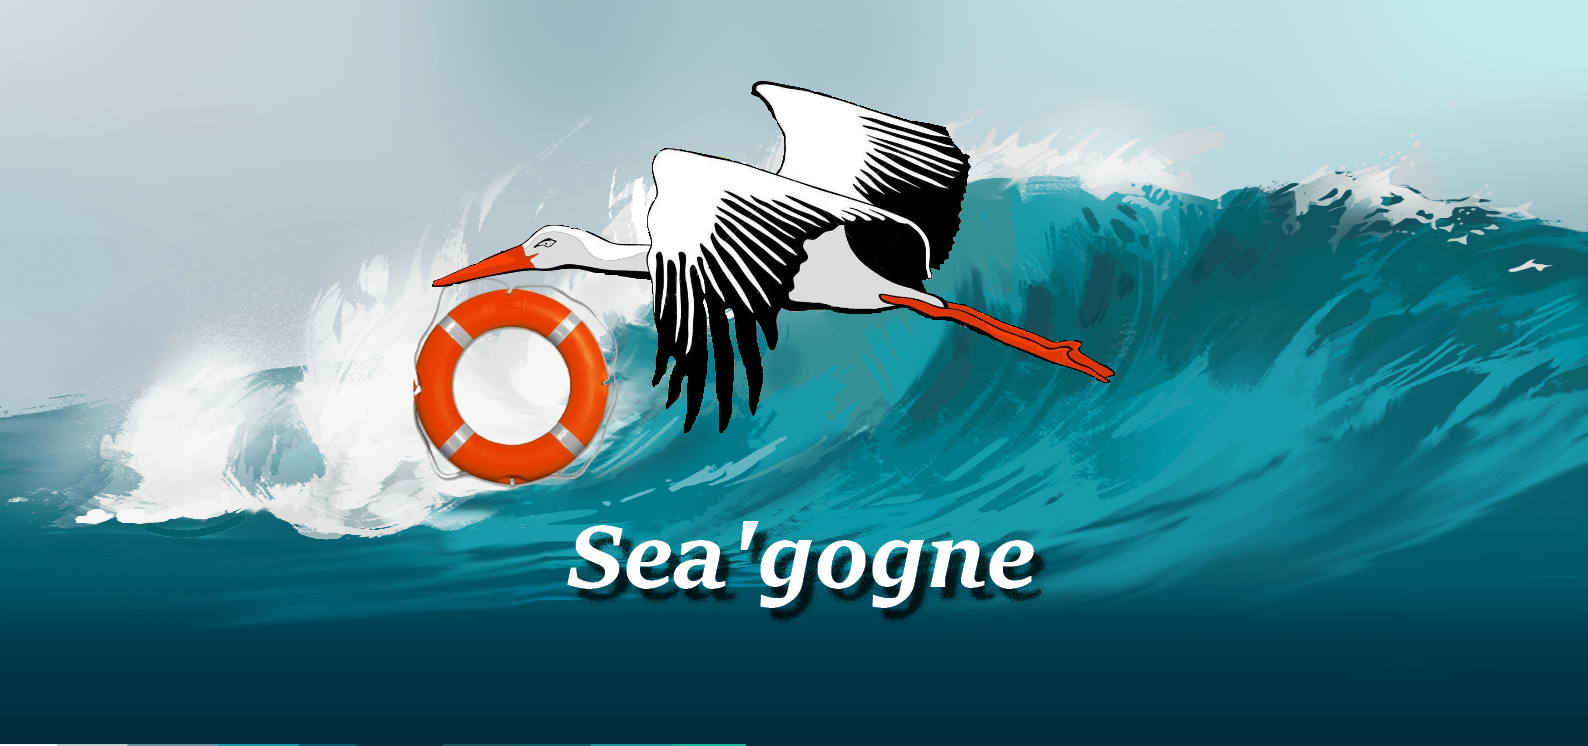
\includegraphics[height=7cm]{figures/seagogne.png}\vskip1cm
        {\large\@author}\vskip2cm
    \end{center}
    \textbf{Professeur référent :}
    \\Monsieur \textsc{Ostre}, Maître de conférence à SeaTech
    \vskip0.5cm
    \centering
    \@date
    \makeatother
\end{titlepage}

\thispagestyle{empty}

\pagenumbering{roman}

\chapter*{Remerciements}

Nous remercions tout d'abord notre professeur référent M.\textsc{Ostre} pour son enthousiasme et ses idées originales tout long de notre projet.\newline

Nous souhaitons également remercier notre école d'ingénieur SeaTech pour les locaux et le matériel à disposition.\newline

Nous remercions tout particulièrement l'équipe encadrante du \textsc{Dassault} UAV Challenge pour l'opportunité qu'ils nous donnent en participant à cette compétition et les dispositifs mis en place pour nous.

%Sommaire
\tableofcontents

\pagenumbering{arabic}

\begin{abstract}
    Dans le cadre de la compétition \textsc{Dassault} UAV Challenge, notre équipe s'attelle à la conception d'un drone VTOL dédié aux opérations de sauvetage en mer. De la sélection de la structure au dimensionnement précis des composants, chaque étape de notre processus de développement est réalisée de manière à créer un drone aussi performant que possible, tout en répondant aux exigences rigoureuses définies par la compétition.

    Grâce à la diversité de nos compétences et à nos recherches approfondies, nous avons fusionné nos connaissances dans le cadre de ce projet pluridisciplinaire. De la modélisation à la simulation, en passant par la programmation, l'automatisation et l'électronique, chaque domaine a été abordé avec une attention particulière. Notre objectif est de présenter un drone qui allie l'expertise technique à une approche globale pour répondre efficacement aux défis complexes du sauvetage en mer. \vskip4cm

    \begin{center}
        \bfseries Abstract
    \end{center}

    \noindent
    \textcolor{red}{traduire}
\end{abstract}

\chapter*{Introduction}
\addcontentsline{toc}{chapter}{\protect\numberline{}Introduction}

Dans le cadre de la compétition organisée par Dassault, nous sommes fiers de présenter notre drone conçu pour répondre à des besoins en sauvetage en mer. Inspiré par l'engagement envers l'innovation et la sécurité, notre équipe a développé un drone à décollage vertical et atterrissage (VTOL) qui redéfinit les normes en matière de missions de sauvetage en milieu maritime.\newline

Face aux défis complexes posés par les situations d'urgence en mer, notre drone VTOL offre une solution polyvalente et efficace. Doté de capacités de décollage vertical, ce drone peut être rapidement déployé depuis diverses plateformes. Sa conception a été minutieusement élaborée pour garantir une performance optimale tout en maintenant une empreinte écologique minimale.\newline

Au-delà de la technologie de pointe, notre drone de sauvetage en mer est équipé de capteurs, d’une caméra et de systèmes de communication. Ces fonctionnalités avancées permettent au drone de localiser rapidement et avec précision les personnes en détresse en mer, fournissant ainsi des informations cruciales pour coordonner des opérations de sauvetage rapides et efficaces.\newline

Nous sommes impatients de démontrer comment notre drone VTOL peut répondre aux exigences et à sa mission de sauvetage en mer. Notre engagement envers l'innovation, la sécurité et l'efficacité se reflète dans chaque aspect de ce projet.


\chapter{Présentation}

\section{Contexte et mission : sauvetage en mer}

Tout d'abord, notre école d'ingénieur SeaTech étant situé à Toulon, première base navale française et premier port de défense d'Europe, et ayant une identité tournée vers le maritime, il nous a paru naturel d'orienter la mission de notre drone vers ce dernier. De plus, sur la côte d'Azur, nous imaginons que les besoins de sauvetage en saison estivale sont amplifiés. C'est pourquoi, nous voulons que notre drone puisse apporter assistance à une personne en mer. Cela passe par sa détection, avec le renvoi d'une coordonnée GPS aux sauveteurs, et par l'assistance d'une bouée de sauvetage en attendant les sauveteurs. Ces informations sont représentées sous un diagramme bête à corne ci-dessous (\ref{bete}).
\bigskip

\begin{figure}[h]
    \centering
    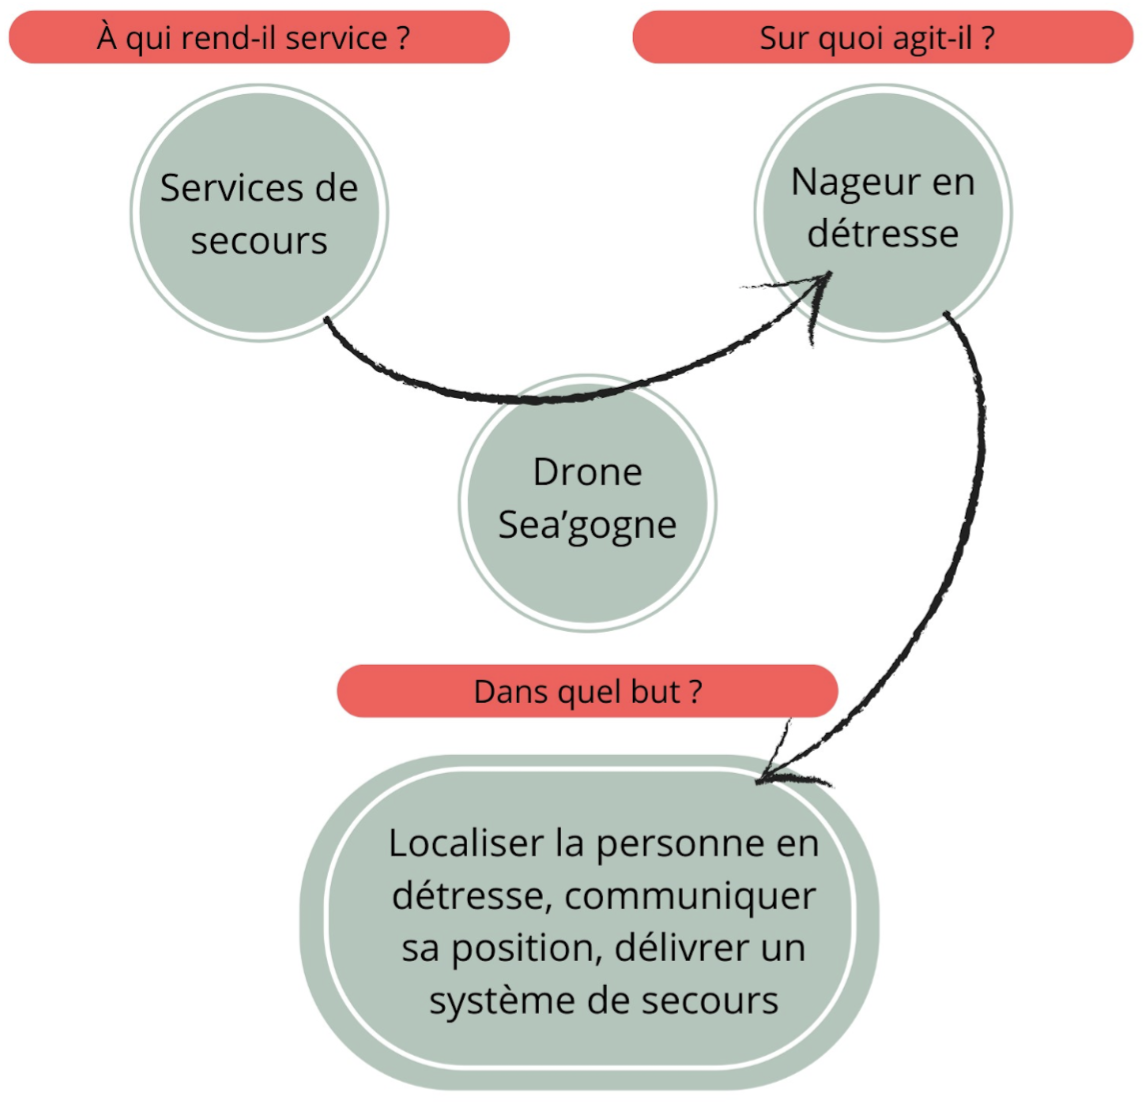
\includegraphics[height=10cm]{figures/bete.png}
    \caption{Diagramme bête à corne}
    \label{bete}
\end{figure}

\section{Fonctionnalités et diagrammes techniques}

\chapter{Réalisation fonctionnelle du drone}

\section{Structure du drone}

Dans cette partie, nous présenterons la structure du drone et les choix qui ont été fait quant à cette dernière.

\subsection{Fuselage}

\subsection{Aile}

\subsubsection*{Profil et dimensionnement des ailes}

Pour le profil de nos deux ailes, nous avons choisi le profil NACA4412. En effet, c'est un profil qui est stable sans décrochage brutal du coefficient de protance (\ref{cz}). D'autre part, dans notre cas d'utilisation, nous ne faisons pas de voltige donc il n'aurait pas été judicieux de prendre un profil symétrique par exemple.

\begin{figure}[h]
    \centering
    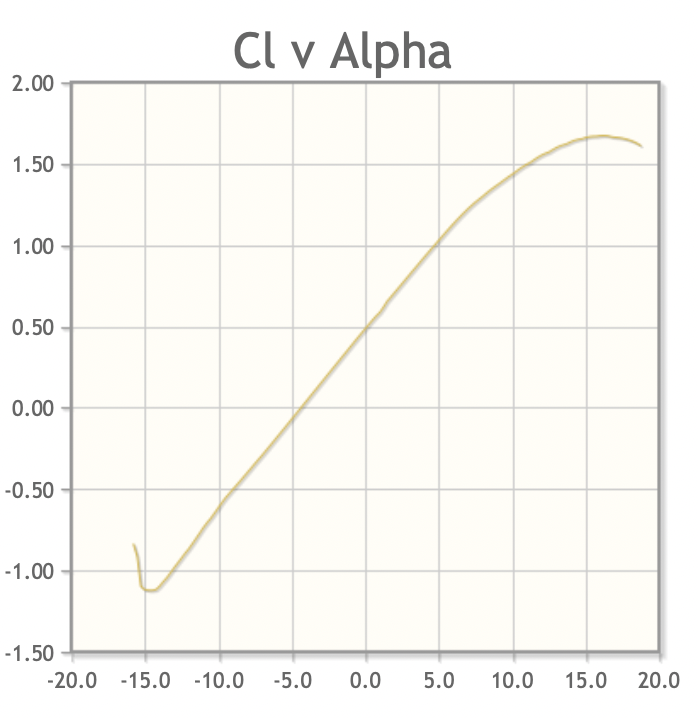
\includegraphics[height=10cm]{figures/cz.png}
    \caption{Courbe du coefficient de portance en fonction de l'incidence}
    \label{cz}
\end{figure}

Nous avons par la suite calculé la surface à l'air de notre aile. Pour cela, nous avons utilisé l'expression de la portance.

$$ F_p=\frac{1}{2}\rho S C_z v^2$$

Avec $C_z$ le coefficient de portance.

Nous déterminons ainsi la surface.
$$S=\frac{2F_p}{\rho C_z v^2}$$

\textcolor{red}{à confirmer}

Nous réalisons les calculs lorsque la force de portance égalise celle du poids du drone : $F_p=P.$ Avec une masse de $m=1$kg, nous trouvons $F_p=9,81$N. Nous choisissons un angle d'incidence de $6°$ ce qui nous donne un coefficient de portance $C_z=1,2$.\newline

Nous trouvons après application numérique une surface de $S=1,265$$m^2$, avec $\rho=1,292$kg/$m^3$ et $v=10$m/s.\newline

    Nous décidons ainsi de dimensionner notre aile de $60cm$ de longeur et $20cm$ de large.

\subsubsection*{Conception de l'aile}

Notre aile est conçu en polystyrène. Elle est découpée à l'aide d'une découpeuse à fil chaud. Après avoir réalisé la modélisation sur Catia du profil de l'aile, nous l'envoyons à la découpeuse.

\textcolor{red}{photo Catia, photo résultat}

\subsection{Systèmes moteur}

\subsection{Structure entre le fuselage et les moteurs : tubes}


\subsection{Empennage}

\section{Contrôle du drone}

\subsection{Système électronique}

\subsection{Interface de commande}

\subsection{Automatisation}

\chapter{Réalisation de la mission : systèmes de sauvetage}

\section{Système de détection}

\section{Système de largage}

\chapter{Estimation du coût }

\chapter{État d'avancement du prototype}

\chapter*{Conclusion}
\addcontentsline{toc}{chapter}{\protect\numberline{}Conclusion}


\end{document}